\documentclass[12pt]{exam}
\usepackage{amsmath}
\usepackage{amsfonts}
\usepackage{graphicx}
% ========== [ End Packages ] ==========


% ==========[ Begin Header ] ==========
\pagestyle{head}
\runningheadrule
\firstpageheadrule
\header{INFO102}{Page \thepage \, sur \numpages}{TP N° 3}
% ==========[ End Header ]==========


% ========== [ Begin Title ] ==========
\title{INFO102 - CR TP N° 3 }
\author{Bellot Ewen}
\date{}
% ========== [ End Title ] ==========


% ========== [ Begin Document ] ==========
\begin{document}
\maketitle
\thispagestyle{head}
\noindent
\tableofcontents
\newpage

\section*{Introduction}
Jeu de casse-briques 2D en JS pur\\
Ce rapport contiens les réponses aux questions/exercices de la deuxième partie du TP N° 3 dand le cadre du module INFO102\\\\
Retrouver le TP ici :\\
\verb|https://developer.mozilla.org/fr/docs/Games/Tutorials/2D_Breakout_game_pure|\\
\verb|_javascript|



\section{Casse-Briques}
\subsection{Créer l'élément Canvas et l'afficher}
Code des 3 fichiers :

\noindent
HTML
\begin{verbatim}
<!doctype html>
<html>
  <head>
    <meta charset="utf-8" />
    <title>Gamedev Canvas Workshop</title>
    <link rel="stylesheet" href="style.css">
    <script async src="script.js"></script>
  </head>
  <body>
    <canvas id="myCanvas" width="480" height="320"></canvas>
  </body>
</html>
\end{verbatim}

\noindent
CSS
\begin{verbatim}
* {
    padding: 0;
    margin: 0;
}
canvas {
    background: #eee;
    display: block;
    margin: 0 auto;
}
\end{verbatim}

\noindent
JS
\begin{verbatim}
var canvas = document.getElementById("myCanvas");
var ctx = canvas.getContext("2d");
\end{verbatim}

\noindent
Triangle\\
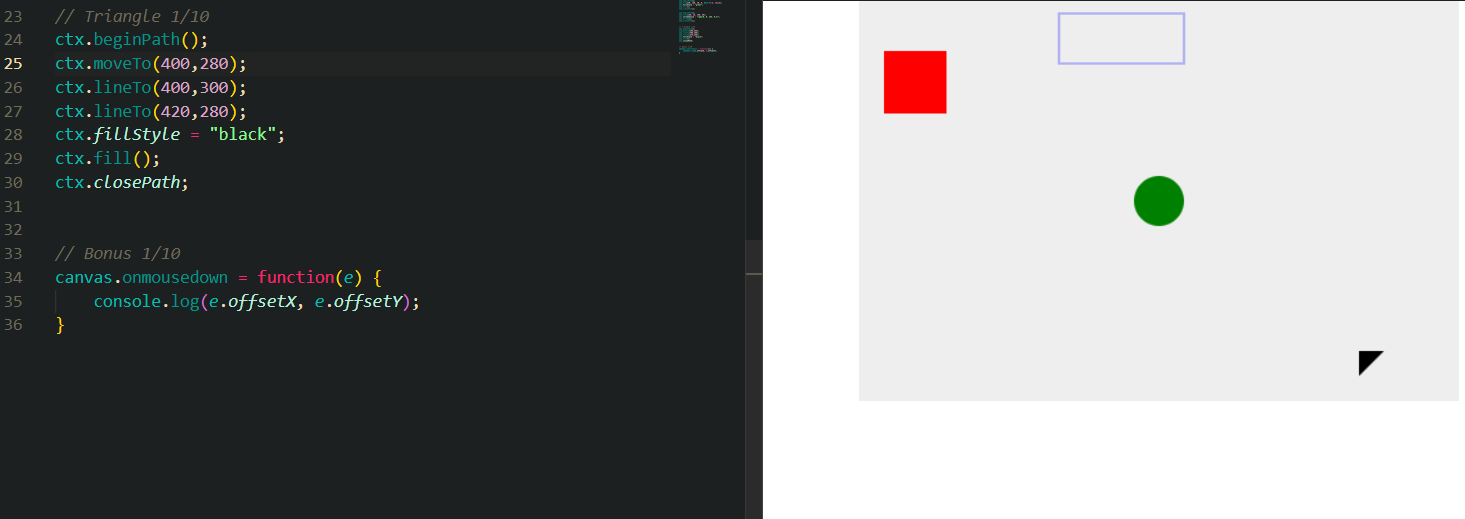
\includegraphics[width=\linewidth]{triangle.png}
\subsection{Déplacer la balle}

Exercice :\\
1. La fonction drawBall dessine la balle, la fonction setInterval(draw, 10) est celle qui apelle a l'infinit la fonction draw, tout les 10 ms.\\
2. Une boucle non bornée pourrait fonctionner avec ce cas précis, mais probablement pas dans la suite des étapes.\\
3. a chaque appel on efface le canvas, puis on change les valeurs de x et y, pour faire bouger la balle.

\subsection{Rebondir contre les murs}
\subsubsection*{\underline{Difference de syntaxe a python}}
la condition du if est placée entre ( parenthèses ), le OR est représenté par $\vert \vert$

J'ai utilisé ce code pour générer un code Hexa aléatoire, pris sur internet.
\begin{verbatim}
    var randomColor = Math.floor(Math.random()*16777215).toString(16);
\end{verbatim}
Le morceau de code génère nombre aléatoire entre 0 et 1, il faut dont le multiplier par un grand nombre, puis l'arrondir a l'unité la plus proche (floor), puis la convertir en chaine de characteres en base 16 (toString(16))

\subsection{Contrôles de clavier}
On ajoute un event listener pour les touches du clavier avec keydown (pressée) et keyup (relachée), on verifie si la touche pressée nous interesse (dans notre cas: m et k, additionelement les touches du pavé directionel aussi) et on assigne un booléen selon notre besoin.\\
Ce booléen est utilisé pour vérifier, a chaque appel de dessin, que la raquette bouge ou non, la direction du mouvement, de plus il y a une restriction pour éviter que la raquette ne sorte du canvas.
 
\subsection{Game Over}


Si la balle entre en collision avec le mur du bas, nous devons vérifier si elle touche la raquette. Si c'est le cas, la balle rebondit et revient dans la zone de jeu. Sinon, le jeu est terminé.

\subsection{Mur de briques}
On définit le nombre de lignes et de colonnes de briques, mais également une hauteur, une largeur et un espacement (padding) entre les briques pour qu'elles ne se touchent pas entre elles et qu'elles ne commencent pas a être tracées sur le bord du canevas. On place nos briques dans un tableau 2D pour représenter leur position, puis on calcule leur position X, y en fonction de la taille d'une brique, du padding, de l'offset a gauche et en haut, mais aussi en fonction du "numéro" de la brique
On les dessine ensuite sur le canvas

Pour ajuster la taille des briques en fonction du nombre de colonnes, il faut utiliser l'equation suivante :
\begin{verbatim}
    var brickWidth = ((canvas.width - (2*brickOffsetLeft))/brickColumnCount)
    - brickPadding;
\end{verbatim}
Cette equation prendre la taille du canvas, lui enlève 60px (dans le cas ou le offset est 30px) pour libérer les 2 coté, puisdivise par le nombre de colonnes pour déterminer ce avec quoi nous travaillons par brique. puis on retire le padding, cette solution nous laisse avec 74px pour une brique avec la disposition originale, a l'instar de 75px comme originalement prévu, cette marge d'erreur étant minime pour les dimentions du projet, nous n'allons pas nous y interesser plus que cela.

\subsection{Détection de collisions}
Nous utilisons une détection de collisions peu sophistiqué, mais amplement suffisante pour notre utilisation du jeux, a partir du centre de la balle, on vérifie la présence ou non de la balle dans la brique, pour cela 4 conditions doivent être remplies :
\begin{verbatim}
    balle.x > brique.x 
    balle.x < brique.x + brickWidth
    balle.y > brique.y
    balle.y < brique.y + brickHeight
\end{verbatim}
Si ces conditions sont remplies, alors la brique disparait.
Par ailleur, pour choisir l'etat de la brique, on vas y attribuer une variable suplémentaire en plus de x et y : status, 0 ou 1, un booléen.\\
si status == 1, on dessine la brique, autrement non. Pour le cas ou on veut dessiner les contours de la brique, on le fait lorsque status == 0 puisque cela signifie que la brique n'as plus lieu d'être.
\newpage
\begin{verbatim}
    var brickX = c * (brickWidth + brickPadding) + brickOffsetLeft;
    var brickY = r * (brickHeight + brickPadding) + brickOffsetTop;
    bricks[c][r].x = brickX;
    bricks[c][r].y = brickY;
    if (bricks[c][r].status == 1) {
        ctx.beginPath();
        ctx.rect(brickX, brickY, brickWidth, brickHeight);
        ctx.fillStyle = "#0095DD";
        ctx.fill();
        ctx.closePath();
    } else { // On dessine les contours ici
        ctx.beginPath();
        ctx.lineWidth = 1;
        ctx.strokeStyle = "#5dc1f3";
        ctx.rect(brickX, brickY, brickWidth, brickHeight);
        ctx.stroke();
        ctx.closePath();
    }
\end{verbatim}

\subsection{Affichage du score et fin de partie (gagné)}
Le score s'incrémente au moment ou l'on a détecté la collision et rendu la brique "cassée", on vérifie par la même occasion si toutes les briques ont été détruites, si tel est le cas, on arrête le jeux de la même façon qu'avec le Game Over, une popup d'alerte et on rafraichit la page. Score++ a été changé en score = score + 2 pour faire gagner plus de points par briques cassés, la poput d'alerte contien aussi le score de la partie lorsqu'on gagne

\subsection{Contrôles de la souris}
Le controle de la sourie inclue une position X relative a la fenetre de jeux et pas seulement a toute la fenetre. On détermine cette position relative en enlevant l'offset du canvas dans la page. Il s'agit ensuite simplement d'aligner le centre de la raquette avec la position X de la sourie. Pour ce qui est des bords, on vérifie que la position relative ne soit pas inferieure a la moitié de la raquette dans le cas de gauche, et superieur a la taille du canvas + la moitié de la raquette dans le cas de droite. comme suit :
\newpage
\begin{verbatim}
function mouseMoveHandler(e) {
    var relativeX = e.clientX - canvas.offsetLeft;
    if (relativeX < (paddleWidth/2)) {
        paddleX = 0;
    } else if (relativeX > (canvas.width-(paddleWidth/2))) {
        paddleX = canvas.width - paddleWidth ;
    } else {
        paddleX = relativeX - paddleWidth / 2;
    }
}
\end{verbatim}

\subsection{Fin}
Le changement en appel récursif au lieu de l'appel toute les 10ms vas permettre au navigateur de dessiner les frames du jeux quand nescessaire plutot que sur un interval fixé, La RAM de l'ordinateur ne peut s'en plaindre.\\
La popup d'alerte en fin de jeu n'est pas idéale, il serait interessant de la remplacer par un bouton pour recommance, qui, quand cliqué, rafraichirait la page.

\end{document}
% ========== [ End Document ] ==========